% Empirical manuscript with held-out Qwen3-0.6B results.

\documentclass[runningheads]{llncs}

\usepackage[T1]{fontenc}
\usepackage{amsmath}
\usepackage{amssymb}
\usepackage{array}
\usepackage{graphicx}
\usepackage{url}
\setlength{\emergencystretch}{2em}

\graphicspath{{../results/qwen3_1_7b_gsm8k_n100_r1/plots/}}

\begin{document}

\title{Adaptive Test-Time Compute for Small Reasoning Models:\\
Held-Out Evaluation of Breadth and Token-Cap Policies}
\titlerunning{Adaptive Test-Time Compute for Small Reasoning Models}

\author{Dinh-Hong Vu\inst{1}\orcidID{0000-0001-8513-3942} \and
The-Tai Phung\inst{2} \and
Thai-Son Bui\inst{2}}

\authorrunning{Dinh-Hong Vu, The Tai Phung and Thai Son Bui}

\institute{Natural Language Processing and Knowledge Discovery Research Group,
Faculty of Information Technology, Ton Duc Thang University,
Ho Chi Minh City, Vietnam\\
\email{vudinhhong@tdtu.edu.vn}
\and
Faculty of Information Technology, Ton Duc Thang University,
Ho Chi Minh City, Vietnam\\
\email{\{52300059,52300058\}@student.tdtu.edu.vn}}

\maketitle

\begin{abstract}
Test-time compute can improve language-model reasoning by extending a single
trajectory or sampling multiple trajectories, but a fixed configuration may
waste computation on easy inputs and remain inadequate for difficult ones. We
study this allocation problem for a small open-weight reasoning model without
an external verifier. Using Qwen3-0.6B, we freeze dataset-specific action
spaces, policies, and 100-problem Test partitions for GSM8K and MATH-500, and
measure exact-answer accuracy, realized generated tokens, latency, validity,
and truncation. On GSM8K, the pre-Test selected agreement-stopping policy at
$L=1024$ attains 76\% accuracy with 1,994.5 mean generated tokens, matching the
accuracy of fixed $k=4,L=1024$ while using 21.3\% fewer tokens. On MATH-500,
the Validation-selected fixed $k=2,L=4096$ policy attains 66\% with 5,141.5
tokens. The frozen joint depth-first heuristic reaches only 36\% with 5,788.8
tokens and is significantly worse than the selected fixed policy. A
breadth-only stopping comparator at $L=4096$ reaches 73\%, equal to fixed
$k=4,L=4096$ in aggregate accuracy while using 20.0\% fewer tokens. Thus the
tested joint heuristic does not provide a consistent cross-dataset Pareto
improvement, whereas dataset-specific fixed and single-axis policies remain
competitive. This negative joint result and the positive adaptive-breadth
results are reported without Test-dependent retuning.

\keywords{Adaptive test-time compute \and Small reasoning models \and
Breadth--depth allocation \and Adaptive inference \and Compute-efficient
reasoning}
\end{abstract}

\section{Introduction}

Reasoning-oriented language models often improve when they spend more
computation at inference time. Computation may be increased by allowing one
trajectory to generate more tokens or by sampling several independent
trajectories and aggregating their answers. Chain-of-thought prompting
\cite{wei2022cot}, self-consistency~\cite{wang2023selfconsistency}, and
repeated-sampling analyses~\cite{brown2024monkeys} demonstrate the value of
these mechanisms, but fixed budgets allocate the same resources to inputs of
different difficulty. Inference-scaling analyses further show that model size,
sampling strategy, and test-time budget jointly determine the
accuracy--compute frontier~\cite{wu2024inference}.

Adaptive inference methods consequently stop sampling when agreement is
sufficient~\cite{aggarwal2023adaptive,wan2025rasc}, estimate difficulty before
allocating samples~\cite{wang2025penny}, or vary the reasoning-token allowance
\cite{han2025token,wu2025thought}. These studies make adaptive allocation an
established research direction. The unresolved question addressed here is
narrower: under resource-constrained local inference, can a lightweight policy
coordinate both a hard token cap and selective resampling for a small
open-weight model, without a learned verifier or access to hidden states?

We operationalize sampling breadth as $k$, the number of independent
trajectories, and use ``depth'' only as shorthand for $L$, the
\texttt{max\_new\_tokens} cap per trajectory. The cap is not a semantic measure
of reasoning depth. We distinguish the nominal budget $kL$ from actual
generated tokens because early stopping and truncation make them empirically
different. Every trajectory acquired by a policy is charged to its realized
cost, including exploratory trajectories that do not determine the final
answer.

Historical Qwen3-1.7B/GSM8K characterization first motivated the working
hypothesis \emph{depth first, breadth selectively}: a usable token allowance
is frequently more valuable than many short, truncated attempts, but a
minority of problems still benefits from additional samples. The primary
Qwen3-0.6B study subsequently evaluates this hypothesis once on frozen
GSM8K and MATH-500 Test partitions, using dataset-specific token-cap grids.

The revised research question is:

\begin{quote}
For small open-weight reasoning models, can a verifier-free lightweight
sequential policy that allocates generation-token caps and selectively adds
independent samples improve the held-out accuracy--actual-generated-token
Pareto frontier over fixed profiles and depth-only or breadth-only adaptive
baselines?
\end{quote}

Supporting questions examine when selective breadth adds value beyond adaptive
depth and whether decisions remain stable across reasoning datasets and a
second small-model family. This study contributes: (i) a reproducible
breadth--token-cap evaluation pipeline with realized-cost accounting and exact
replay; (ii) held-out comparisons of 14 registered policies on GSM8K and
MATH-500; (iii) evidence that agreement-based breadth stopping can preserve
the accuracy of fixed high-breadth comparators while reducing generated
tokens; and (iv) a cross-dataset result showing that the evaluated joint
heuristic does not generalize reliably. The Train data did not contain enough
positive escalation events to fit a learned joint controller, so the joint
policy evaluated here is a deterministic heuristic.

\section{Related Work}

\subsection{Test-Time Scaling and Self-Consistency}

Chain-of-thought prompting elicits intermediate reasoning before the final
answer~\cite{wei2022cot}. Self-consistency samples several reasoning paths and
selects the most frequent answer~\cite{wang2023selfconsistency}. Repeated
sampling can increase solution coverage, although converting coverage into
final-answer accuracy may require effective selection or verification
\cite{brown2024monkeys}. These methods establish breadth as one test-time
compute axis but normally use a preset sample count.

\subsection{Adaptive Sampling and Early Stopping}

Adaptive-Consistency stops sampling when the answer distribution stabilizes
\cite{aggarwal2023adaptive}. Difficulty-Adaptive Self-Consistency combines
prior difficulty estimates with posterior evidence~\cite{wang2025penny}.
Reasoning-Aware Self-Consistency evaluates both answers and rationales when
stopping and aggregating~\cite{wan2025rasc}. These are direct precedents for
adaptive breadth. Early-Stopping Self-Consistency (ESC) likewise terminates
sampling after sufficient answer agreement~\cite{li2024esc}, while Certaindex
uses answer stabilization to signal that further reasoning compute is unlikely
to change the result~\cite{fu2025certaindex}. Our agreement-stopping baseline
is intentionally simpler: it uses exact normalized-answer agreement and at
most four independent samples.

\subsection{Adaptive Token Budgets}

Token-Budget-Aware LLM Reasoning assigns budgets according to estimated
complexity~\cite{han2025token}. Thought Calibration uses probes over hidden
representations to detect when further reasoning is unlikely to help
\cite{wu2025thought}. More general approaches learn input-dependent allocation
of inference computation~\cite{snell2025scaling,damani2025hard}. The s1 study
controls reasoning length through budget forcing~\cite{muennighoff2025s1}, and
L1 learns prompt-conditioned length control with reinforcement
learning~\cite{aggarwal2025l1}. These methods also show that a hard generation
cutoff is only one way to impose a budget. Our experiments use an unmodified
Qwen3 decoder and therefore do not test forced-answer decoding or learned
length control.

Longer reasoning is not uniformly beneficial. ``When More is Less'' reports
an inverted-U relation between chain-of-thought length and accuracy in several
settings~\cite{wu2025moreless}. This motivates reporting observed token use and
truncation rather than treating $L$ as semantic reasoning depth.

\subsection{Difficulty-Aware Learned Allocation}

Difficulty prediction has been used to choose sample counts and allocate
average budgets across a problem set~\cite{wang2025penny,zhai2026adaptive}.
Strong oracle gaps do not imply that oracle actions can be predicted from
cheap features. We therefore evaluate policy accuracy and realized cost
directly instead of treating profile-label classification as the scientific
endpoint.

\subsection{Joint Parallel--Sequential Compute}

Parallel and sequential computation can complement one another. PaCoRe, for
example, coordinates parallel trajectories across multiple rounds through
message passing~\cite{hu2026pacore}. That approach relies on specialized
training and synthesis at a much larger scale. Our evaluated policy family
instead targets local, small-model inference and chooses whether to purchase
another independent trajectory after observing only signals already produced
by the current policy.

\subsection{Efficient Reasoning for Small Models}

Budget-aware evaluation is essential because a more elaborate strategy can
appear better simply by consuming more computation~\cite{wang2024tokeneconomies}.
Small open-weight models make this accounting especially relevant under a
single-GPU constraint. Qwen3 provides suitable open-weight model sizes for the
study~\cite{qwen3report}; however, results from its 1.7B and 0.6B variants are
kept as separate strata rather than pooled into a model-family claim.

\subsection{Position of This Study}

This study investigates joint breadth--token-cap allocation under four
constraints: a small open-weight model, no external verifier, strict
final-answer parsing, and realized-token cost accounting. Fixed profiles,
adaptive breadth, adaptive depth, and a deterministic joint heuristic are
compared on two held-out datasets.

\section{Problem Formulation}

Let $x_i$ be a reasoning problem with ground-truth answer $y_i$. An inference
profile is
\begin{equation}
  p=(k,L)\in\mathcal{P},
\end{equation}
where $k$ is the number of independent trajectories and $L$ is the maximum
number of newly generated tokens per trajectory. Its nominal budget is
$B(p)=kL$, whereas realized generated-token cost is
\begin{equation}
  C_i(p)=\sum_{j=1}^{k} t_{ij}(L), \qquad t_{ij}(L)\leq L.
\end{equation}

Each trajectory is parsed using a strict final-answer extractor. Let $V_i(p)$
be the multiset of valid normalized answers. If $V_i(p)$ is non-empty, the
system returns the majority answer with a deterministic lowest-sample-index
tie break. Invalid answers do not vote; a profile with no valid answer is
incorrect. Final correctness is denoted by $A_i(p)\in\{0,1\}$.

Let $\mathcal{S}_i=\{p\in\mathcal{P}:A_i(p)=1\}$ and let
$r_i(p)=(C_i(p),T_i(p),B(p),k,L)$. The retrospective joint-oracle selection is
\begin{equation}
  p_i^{*}=\arg\min_{p\in\mathcal{S}_i} r_i(p),
  \qquad \mathcal{S}_i\neq\varnothing.
\end{equation}
where $T_i(p)$ is latency and the tuple defines deterministic tie breaking.
If $\mathcal{S}_i$ is empty, we instead set
$p_i^{*}=\arg\min_{p\in\mathcal{P}}r_i(p)$. This rule charges an unsolved
problem for its cheapest observed candidate rather than removing it from the
cost denominator. The oracle sees
ground-truth outcomes from the complete realized sample pool and is therefore
an opportunity bound conditional on one stochastic generation seed.

The evaluated policies do not estimate a probability of correctness and do
not optimize a fitted $\lambda$-weighted utility. They are deterministic rules
defined in Section~\ref{sec:policies}. During replay, a policy can use the
input and outputs it has already generated; it cannot use ground truth,
oracle labels, future samples, or counterfactual outcomes.

\section{Experimental Framework}

\subsection{System Architecture and Reproducibility}

Figure~\ref{fig:architecture} summarizes the implemented pipeline and the
boundary between frozen deployable signals and retrospective analysis.

\begin{figure}
\centering
\fbox{\begin{minipage}{0.91\textwidth}
\centering
\textbf{Frozen dataset manifest and model revision}\\[2mm]
$\downarrow$\\[-1mm]
\textbf{Dataset/model adapters $\rightarrow$ deterministic seeds
$\rightarrow$ append-only generation cache}\\[2mm]
$\downarrow$\\[-1mm]
\textbf{Strict parser $\rightarrow$ valid-only aggregation
$\rightarrow$ correctness, tokens, latency, truncation}\\[2mm]
$\downarrow$\\[-1mm]
\textbf{Frozen fixed, depth-only, breadth-only, and joint-heuristic replay}\\[2mm]
$\downarrow$\\[-1mm]
\textbf{One-shot held-out comparison and paired statistical analysis}
\end{minipage}}
\caption{Evaluation pipeline. Train data determine policy thresholds,
Validation selects a registered operating point, and the selected policy and
all comparators are replayed once on the held-out Test partition.}
\label{fig:architecture}
\end{figure}

For the completed grid, samples are nested within a token cap: $k=1$ uses
sample 0, $k=2$ uses samples 0--1, and $k=4$ uses samples 0--3. Thus each
problem requires twelve unique generations rather than independently
regenerating all nine profiles. Seeds depend on the global seed, problem ID,
repetition ID, and sample ID, not on $k$ or $L$. The system separates adapters,
strict parsing, generation, checkpoint/resume, provenance manifests, cost
accounting, controller-data construction, and statistical reporting.

\subsection{Answer Parsing and Aggregation}

The parser accepts explicit numeric final-answer formats, including GSM8K
markers, boxed answers, and explicit final-answer fields. It does not use the
last number in free-form reasoning as a fallback. Responses are categorized as
truncated during thinking, truncated after thinking, completed but
unparseable, or completed with a valid answer. One selected GSM8K record was
flagged for manual review; it remains in raw artifacts but is excluded from
accuracy, Pareto, and oracle metrics. Benchmark labels are not rewritten.

\subsection{Models, Data, and Splits}

The historical characterization uses Qwen3-1.7B revision
\texttt{70d244cc} (full revision in the manifest) and the GSM8K test split
\cite{cobbe2021gsm8k}. Generation uses thinking mode, temperature 0.7,
top-$p$ 0.95, CUDA, and bfloat16. A seed-42 manifest contains 100 problems; 99
contribute to main metrics after the audit exclusion. The grid contains 1,200
unique generation records from one stochastic repetition.

The primary study uses Qwen3-0.6B revision
\texttt{c1899de2} (full revision in the manifest) after an 8192-token 1.7B
diagnostic proved infeasible on the available RTX 4060. This amendment does
not relabel or pool 1.7B evidence. Generation uses thinking mode, temperature
0.7, top-$p$ 0.95, CUDA, bfloat16, and seed 42. GSM8K uses prompt
\path{gsm8k_cot_v3}, parser \path{gsm8k_numeric_v3}, and
$L\in\{512,1024,2048\}$. MATH-500~\cite{hendrycks2021math} uses prompt
\path{math500_cot_v1}, parser \path{math500_exact_v2}, and
$L\in\{1024,2048,4096\}$. Both use $k\in\{1,2,4\}$.

The frozen GSM8K manifest contains 79 Train, 20 Validation, and 100 disjoint
Test problems. The MATH-500 manifest contains 80 Train, 20 Validation, and 100
disjoint Test problems, stratified by subject and difficulty. Validation is
used for selection and pivot decisions, never as final evidence. After policy
and software freezing, each Test grid was generated once, producing all 1,200
expected records without generation errors, missing keys, or duplicates. Test
outcomes were not used to refit or replace a frozen policy.

\subsection{Metrics and Statistical Analysis}

Primary outcomes are exact final-answer accuracy and actual generated tokens.
Secondary metrics are nominal $kL$, latency, truncation, valid-answer fraction,
and tokens per correct answer. Accuracy uses Wilson 95\% intervals. Planned
depth, breadth, and equal-budget comparisons use exact paired McNemar tests
with Holm correction within pre-specified families. Problem-level paired
bootstrap intervals summarize policy accuracy and token differences. Pareto
status is descriptive on Test and never used for post-Test reselection. One
repetition measures variation over problems but not generation-seed
variability.

\section{Historical Oracle Breadth--Depth Characterization}

The completed characterization evaluates nine profiles with breadths
$\{1,2,4\}$ and token caps $\{512,1024,2048\}$. Figure~\ref{fig:heatmap} and
Table~\ref{tab:grid} show a strong token-cap effect at every breadth. All six
adjacent depth comparisons are significant after Holm correction. Four of six
adjacent breadth comparisons are significant; the $k=2$ to $k=4$ comparisons
at $L=1024$ and $L=2048$ are inconclusive.

\begin{figure}
\centering
\includegraphics[width=0.72\textwidth]{accuracy_heatmap.png}
\caption{Completed Qwen3-1.7B/GSM8K accuracy characterization on 99 usable
problems. Values describe the tested setting and one stochastic repetition.}
\label{fig:heatmap}
\end{figure}

\begin{table}
\caption{Final-answer accuracy on 99 evaluated GSM8K problems.}
\label{tab:grid}
\centering
\begin{tabular}{c|ccc}
\hline
$k$ & $L=512$ & $L=1024$ & $L=2048$ \\
\hline
1 & 9.09\% & 53.54\% & 70.71\% \\
2 & 17.17\% & 65.66\% & 81.82\% \\
4 & 28.28\% & 71.72\% & 83.84\% \\
\hline
\end{tabular}
\end{table}

At equal nominal budget $kL=2048$, the configurations behave differently
(Table~\ref{tab:isobudget}). Four short trajectories are heavily truncated;
one long trajectory is more accurate and consumes fewer realized tokens. This
supports the operational hypothesis but does not establish universal depth
dominance.

\begin{table}
\caption{Profiles with equal nominal budget $kL=2048$.}
\label{tab:isobudget}
\centering
\begin{tabular}{c|r|r|r}
\hline
Profile & Accuracy & Avg. actual tokens & Sample truncation \\
\hline
$4\times512$ & 28.28\% & 1,988.9 & 85.4\% \\
$2\times1024$ & 65.66\% & 1,616.0 & 35.9\% \\
$1\times2048$ & 70.71\% & 1,079.1 & 18.2\% \\
\hline
\end{tabular}
\end{table}

The joint cheapest-correct oracle solves 83 of 99 problems. Seventy select a
$k=1$ profile; 13 require $k>1$ under the observed sample pool. Fifty-five
select $L=2048$, and none selects $L=512$ as cheapest-correct. This imbalance
argues against a flat nine-class controller and motivates staged escalation
decisions.

Figure~\ref{fig:pareto} shows the observed fixed-profile frontier, while
Table~\ref{tab:oracle} quantifies retrospective adaptive headroom. The best
fixed profile solves 83 problems at 4,246.7 tokens per
problem. The joint oracle matches that accuracy at 1,023.5 tokens. At
approximately this realized cost, the exact budget-constrained frontier solves
83 problems for joint allocation, 70 for depth-only, 69 for breadth-only, and
53 for fixed allocation. The 13.13-point joint-versus-depth oracle gap is an
opportunity estimate, not controller evidence.

\begin{figure}
\centering
\includegraphics[width=0.76\textwidth]{pareto.png}
\caption{Observed fixed-profile accuracy--realized-token frontier. Oracle
anchors are reported separately in Table~\ref{tab:oracle}.}
\label{fig:pareto}
\end{figure}

\begin{table}
\caption{Fixed and retrospective oracle anchors.}
\label{tab:oracle}
\centering
\begin{tabular}{l|l|r|r|r}
\hline
Strategy & Anchor & Solved & Accuracy & Avg. tokens \\
\hline
Fixed & $4\times2048$ & 83 & 83.84\% & 4,246.7 \\
Breadth-only oracle & $L=2048$ & 83 & 83.84\% & 1,270.6 \\
Depth-only oracle & $k=1$ & 70 & 70.71\% & 750.5 \\
Depth-only oracle & $k=4$ & 83 & 83.84\% & 3,118.1 \\
Joint oracle & all profiles & 83 & 83.84\% & 1,023.5 \\
\hline
\end{tabular}
\end{table}

\section{Evaluated Allocation Policies}
\label{sec:policies}

\subsection{Policy Definitions}

Each policy uses the input and signals from trajectories already generated and
charged to its cost. The input-only depth policy maps Train-fitted prompt-token
tertiles to an $L$ action and always uses $k=1$. The breadth-only policy fixes
$L$, acquires two samples, stops when both parsed answers are valid and equal,
and otherwise acquires samples 3--4. Fixed policies evaluate every $(k,L)$
pair.

The joint depth-first heuristic first maps Train prompt-token tertiles to $L$.
It stops at $k=1$ only for a valid, non-truncated final answer, stops at $k=2$
only when two valid answers agree, and otherwise acquires $k=4$. Every paid
trajectory contributes to actual generated-token cost, including invalid,
truncated, or discarded samples. The same policy code reconstructs fixed
endpoints exactly before adaptive results are accepted.

\subsection{Policy Selection}

Fitting a learned joint controller required at least 30 positive Train
escalation events per stage. The observed Train split did not meet this
threshold. We therefore evaluated the registered deterministic heuristic and
do not report a learned-controller result.

On GSM8K Validation, agreement stopping at $L=1024$ and the joint heuristic
both solve 15/20 problems; agreement stopping uses 2,095.85 rather than
2,149.05 mean tokens and wins the pre-Test tie-break. On MATH-500 Validation,
every adaptive policy is point-dominated: fixed $k=2,L=4096$ solves 13/20 at
4,700.50 tokens, whereas the joint heuristic solves 10/20 at 5,935.55 tokens.
The fixed MATH policy was consequently selected after Validation and before
Test evaluation.

The selected policies, all 14 comparators, action spaces, prompts, parsers,
Train thresholds, seeds, and software hashes were serialized before Test
access. GSM8K and MATH-500 were then evaluated once and separately. The
selection rule was not reopened after observing Test results.

\section{Experimental Results}

Table~\ref{tab:testpolicies} reports the main held-out operating points.
Figure~\ref{fig:testpolicyfrontiers} shows the complete 14-policy
accuracy--compute trade-off for each dataset.

\begin{table}
\caption{Frozen Qwen3-0.6B Test policy results. ``Selected'' denotes the
policy fixed before its dataset's Test outcomes were accessed.}
\label{tab:testpolicies}
\centering
\small
\begin{tabular}{l|>{\raggedright\arraybackslash}p{4.2cm}|r|r|c}
\hline
Data & Policy & Correct & Avg. tokens & Frontier \\
\hline
GSM8K & breadth stop, $L=1024$ (selected) & 76/100 & 1,994.52 & yes \\
GSM8K & joint heuristic & 70/100 & 1,449.46 & yes \\
GSM8K & fixed $2\times2048$ & 71/100 & 1,603.00 & yes \\
GSM8K & fixed $4\times1024$ & 76/100 & 2,535.17 & no \\
\hline
MATH & fixed $2\times4096$ (selected) & 66/100 & 5,141.50 & yes \\
MATH & joint heuristic & 36/100 & 5,788.81 & no \\
MATH & breadth stop, $L=4096$ & 73/100 & 8,191.12 & yes \\
MATH & fixed $4\times4096$ & 73/100 & 10,233.17 & no \\
\hline
\end{tabular}
\end{table}

\begin{figure}
\centering
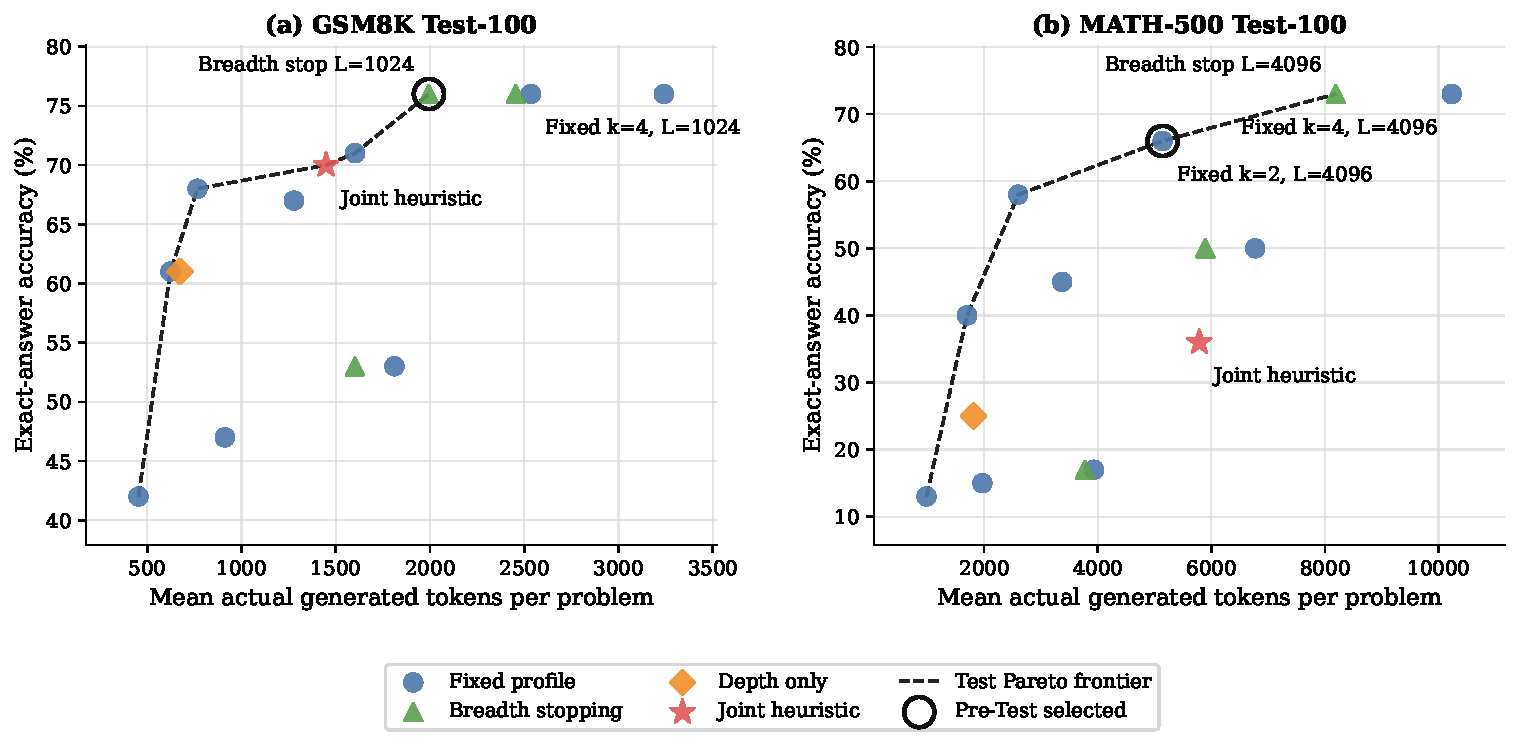
\includegraphics[width=\textwidth]{figures/cross_dataset_test_policy_pareto.pdf}
\caption{Frozen Test accuracy versus mean actual generated tokens for all 14
registered policies per dataset. Dashed lines show descriptive Test Pareto
frontiers, and black rings mark the policies selected before Test access.
Frontier membership is not used for post-Test policy reselection.}
\label{fig:testpolicyfrontiers}
\end{figure}

\subsection{GSM8K Held-Out Result}

The frozen selected breadth policy attains 76\% accuracy (Wilson 95\% CI
[66.8\%, 83.3\%]) and stops at $k=2$ on 54 problems. Relative to fixed
$k=4,L=1024$, it has the same correct/incorrect outcome on every Test problem
while reducing mean generated tokens from 2,535.17 to 1,994.52, a 21.3\%
reduction. This is the clearest held-out efficiency result.

The joint heuristic attains 70\% (95\% CI [60.4\%, 78.1\%]) at 1,449.46
tokens. Compared with the selected policy, it loses six accuracy points and
saves 545.06 tokens. Seven discordant problems favor the selected policy and
one favors the joint heuristic; the exact McNemar $p=0.0703$ and
Holm-adjusted $p=0.4922$ are inconclusive. Both policies therefore remain on
the descriptive Test frontier, and the Validation selection is not reopened.

\subsection{MATH-500 Held-Out Result}

The frozen selected fixed $k=2,L=4096$ policy attains 66\% accuracy (Wilson
95\% CI [56.3\%, 74.5\%]) at 5,141.50 tokens, close to its 65\% Validation
estimate. The joint heuristic attains 36\% (95\% CI [27.3\%, 45.8\%]) at
5,788.81 tokens. Its paired accuracy difference relative to the selected
policy is $-30$ points, with Holm-adjusted exact McNemar
$p=2.50\times10^{-6}$. It is also point-dominated by fixed $k=1,L=4096$,
which attains 58\% at 2,600.28 tokens.

The breadth-only stopping comparator at $L=4096$ attains 73\% (95\% CI
[63.6\%, 80.7\%]) at 8,191.12 tokens. This equals the aggregate accuracy of
fixed $k=4,L=4096$ while reducing mean tokens by 19.96\% and recorded latency
by 19.44\%. This registered comparator is reported as a secondary result; the
Validation-selected fixed policy remains the primary MATH operating point.

\subsection{Cross-Dataset Comparison}

The joint heuristic is a lower-cost Pareto point on GSM8K but is decisively
dominated on MATH-500. The result does not support a common joint allocation
rule across the two datasets. Dataset-specific fixed or single-axis policies
provide stronger operating points, while the adaptive-breadth findings remain
positive on both datasets.

\section{Discussion}

Across both datasets, adequate token cap is important: many short samples
cannot compensate for severe truncation. Breadth nevertheless remains useful.
Agreement stopping removes unnecessary later samples on GSM8K, and at
$L=4096$ it preserves the best aggregate MATH-500 accuracy while using less
compute than fixed $k=4$. The useful operating point is dataset-dependent:
GSM8K selects adaptive breadth at moderate depth, whereas MATH Validation
selects a fixed $k=2$ high-depth profile.

Retrospective joint-oracle headroom did not translate into a stable cheap
heuristic across datasets. On
MATH-500, the trace pattern suggests that prompt-length tertiles often choose
insufficient caps, while later validity/agreement escalation cannot recover
the resulting accuracy. Oracle headroom therefore overstates what the tested
input-only heuristic can realize.

The selected GSM8K and MATH policies are evaluated on different tasks and
token-cap grids and are therefore not directly comparable. The MATH breadth
comparator has higher Test accuracy, but the Validation-selected fixed policy
remains the primary estimate. Frozen manifests, versioned prompts and parsers,
nested sample reuse, resumable generation, exact replay, and source hashes
record the selection and evaluation sequence.

\section{Limitations and Future Evaluation}

The results are bounded by the following design choices:
\begin{itemize}
  \item each held-out dataset contains 100 Test problems and one
  stochastic generation seed;
  \item the primary evidence covers one 0.6B model from one model family;
  \item $L$ is a token cap and cannot be interpreted as semantic reasoning
  depth;
  \item the oracle is computed from the same one-seed sample pool, so a
  lucky correct trajectory can make its estimated headroom optimistic;
  \item each 20-problem Validation partition gives a noisy policy-selection
  estimate, and the MATH fixed-policy pivot was registered after Validation;
  \item the available Train splits did not meet the minimum positive
  Train-event requirement for a learned joint controller;
  \item generation uses Qwen3 thinking mode with hard
  \texttt{max\_new\_tokens} caps. Budget forcing, Qwen3's native
  thinking-budget interface, and non-thinking mode were not evaluated, so
  truncation-sensitive comparisons cannot isolate semantic reasoning depth;
  \item the 1.7B MATH-500 run was not completed because the required long
  context was infeasible on the available RTX 4060; the 1.7B evidence is
  therefore limited to GSM8K and is not pooled with the 0.6B study;
  \item recorded latency is hardware- and execution-specific;
  \item Test Pareto membership is descriptive and was not used for policy
  reselection.
\end{itemize}

Repeated seeds are needed to estimate generation variability. The three
decoding controls above would determine how much of the historical token-cap
effect comes from forced truncation rather than useful deliberation. A learned
joint controller would additionally require more Train escalation events and a
new untouched Test partition; the current Test outcomes cannot support further
tuning.

\section{Conclusion}

Frozen Qwen3-0.6B evaluation shows that no single joint allocation rule is
reliably best across GSM8K and MATH-500. The tested joint heuristic remains a
lower-cost Pareto point on GSM8K but is significantly worse and more expensive
than the selected fixed policy on MATH-500. The cross-dataset joint hypothesis
is therefore not supported. In contrast, agreement-based breadth stopping
provides concrete efficiency gains: it reduces GSM8K tokens by 21.3\% with
identical paired correctness to fixed $k=4,L=1024$, and reduces MATH-500 tokens
by 20.0\% at the same aggregate accuracy as fixed $k=4,L=4096$. These results
support dataset-specific fixed and single-axis allocation, with explicit
realized-cost accounting and no Test-dependent retuning.

\appendix
\makeatletter
\setlength{\@fptop}{0pt}
\makeatother
\section{Complete Frozen Test Policy Results}

Tables~\ref{tab:gsmallpolicies} and~\ref{tab:mathallpolicies} report every
registered replay policy underlying Figure~\ref{fig:testpolicyfrontiers}.
The word ``selected'' marks the policy chosen using Validation before Test access.
The frontier column is a descriptive summary of the held-out results and was
not used to revise either selection.

\begin{table}[!ht]
\caption{Complete GSM8K frozen Test replay ($n=100$), ordered by mean actual
generated tokens.}
\label{tab:gsmallpolicies}
\centering
\small
\begin{tabular}{l|r|r|c}
\hline
Policy & Accuracy & Avg. tokens & Frontier \\
\hline
Fixed $k=1,L=512$ & 42\% & 454.31 & yes \\
Fixed $k=1,L=1024$ & 61\% & 623.19 & yes \\
Depth only & 61\% & 673.67 & no \\
Fixed $k=1,L=2048$ & 68\% & 767.15 & yes \\
Fixed $k=2,L=512$ & 47\% & 912.46 & no \\
Fixed $k=2,L=1024$ & 67\% & 1,278.53 & no \\
Joint heuristic & 70\% & 1,449.46 & yes \\
Breadth stop, $L=512$ & 53\% & 1,601.83 & no \\
Fixed $k=2,L=2048$ & 71\% & 1,603.00 & yes \\
Fixed $k=4,L=512$ & 53\% & 1,811.51 & no \\
Breadth stop, $L=1024$ (selected) & 76\% & 1,994.52 & yes \\
Breadth stop, $L=2048$ & 76\% & 2,455.01 & no \\
Fixed $k=4,L=1024$ & 76\% & 2,535.17 & no \\
Fixed $k=4,L=2048$ & 76\% & 3,240.74 & no \\
\hline
\end{tabular}
\end{table}

\begin{table}[!ht]
\caption{Complete MATH-500 frozen Test replay ($n=100$), ordered by mean
actual generated tokens.}
\label{tab:mathallpolicies}
\centering
\small
\begin{tabular}{l|r|r|c}
\hline
Policy & Accuracy & Avg. tokens & Frontier \\
\hline
Fixed $k=1,L=1024$ & 13\% & 984.67 & yes \\
Fixed $k=1,L=2048$ & 40\% & 1,699.27 & yes \\
Depth only & 25\% & 1,813.19 & no \\
Fixed $k=2,L=1024$ & 15\% & 1,968.96 & no \\
Fixed $k=1,L=4096$ & 58\% & 2,600.28 & yes \\
Fixed $k=2,L=2048$ & 45\% & 3,374.69 & no \\
Breadth stop, $L=1024$ & 17\% & 3,776.01 & no \\
Fixed $k=4,L=1024$ & 17\% & 3,933.58 & no \\
Fixed $k=2,L=4096$ (selected) & 66\% & 5,141.50 & yes \\
Joint heuristic & 36\% & 5,788.81 & no \\
Breadth stop, $L=2048$ & 50\% & 5,894.19 & no \\
Fixed $k=4,L=2048$ & 50\% & 6,772.25 & no \\
Breadth stop, $L=4096$ & 73\% & 8,191.12 & yes \\
Fixed $k=4,L=4096$ & 73\% & 10,233.17 & no \\
\hline
\end{tabular}
\end{table}

\clearpage
\section{Historical Grid Uncertainty}

Table~\ref{tab:historicalci} reports Wilson intervals for the nine historical
Qwen3-1.7B/GSM8K profiles. Table~\ref{tab:historicalmcnemar} gives every
pre-specified adjacent depth, adjacent breadth, and equal-budget comparison.
Holm correction is applied within each comparison family.

\begin{table}[!ht]
\caption{Historical Qwen3-1.7B/GSM8K accuracy with Wilson 95\% intervals
($n=99$).}
\label{tab:historicalci}
\centering
\small
\begin{tabular}{c|c|r|c}
\hline
$k$ & $L$ & Accuracy & Wilson 95\% CI \\
\hline
1 & 512  & 9.1\%  & [4.9\%, 16.4\%] \\
1 & 1024 & 53.5\% & [43.8\%, 63.0\%] \\
1 & 2048 & 70.7\% & [61.1\%, 78.8\%] \\
2 & 512  & 17.2\% & [11.0\%, 25.8\%] \\
2 & 1024 & 65.7\% & [55.9\%, 74.3\%] \\
2 & 2048 & 81.8\% & [73.1\%, 88.2\%] \\
4 & 512  & 28.3\% & [20.4\%, 37.8\%] \\
4 & 1024 & 71.7\% & [62.2\%, 79.6\%] \\
4 & 2048 & 83.8\% & [75.3\%, 89.8\%] \\
\hline
\end{tabular}
\end{table}

\begin{table}[!ht]
\caption{Exact paired McNemar tests for the historical grid ($n=99$).
$A$-only and $B$-only are discordant correctness counts; ``inc.'' denotes an
inconclusive family-wise result at $\alpha=0.05$.}
\label{tab:historicalmcnemar}
\centering
\small
\begin{tabular}{l|l|r|r|r|r|c}
\hline
Family & $A\rightarrow B$ & $A$-only & $B$-only & Exact $p$ & Holm $p$ & Result \\
\hline
Depth & $1{\times}512\rightarrow1{\times}1024$ & 0 & 44 & 1.14e-13 & 5.68e-13 & sig. \\
Depth & $1{\times}1024\rightarrow1{\times}2048$ & 0 & 17 & 1.53e-5 & 4.58e-5 & sig. \\
Depth & $2{\times}512\rightarrow2{\times}1024$ & 0 & 48 & 7.11e-15 & 4.26e-14 & sig. \\
Depth & $2{\times}1024\rightarrow2{\times}2048$ & 0 & 16 & 3.05e-5 & 6.10e-5 & sig. \\
Depth & $4{\times}512\rightarrow4{\times}1024$ & 0 & 43 & 2.27e-13 & 9.09e-13 & sig. \\
Depth & $4{\times}1024\rightarrow4{\times}2048$ & 0 & 12 & 4.88e-4 & 4.88e-4 & sig. \\
\hline
Breadth & $1{\times}512\rightarrow2{\times}512$ & 0 & 8 & 0.0078 & 0.0234 & sig. \\
Breadth & $2{\times}512\rightarrow4{\times}512$ & 0 & 11 & 0.0010 & 0.0049 & sig. \\
Breadth & $1{\times}1024\rightarrow2{\times}1024$ & 0 & 12 & 0.0005 & 0.0029 & sig. \\
Breadth & $2{\times}1024\rightarrow4{\times}1024$ & 0 & 6 & 0.0313 & 0.0625 & inc. \\
Breadth & $1{\times}2048\rightarrow2{\times}2048$ & 0 & 11 & 0.0010 & 0.0049 & sig. \\
Breadth & $2{\times}2048\rightarrow4{\times}2048$ & 0 & 2 & 0.5000 & 0.5000 & inc. \\
\hline
Equal budget & $4{\times}512\rightarrow2{\times}1024$ & 1 & 38 & 1.46e-10 & 3.94e-10 & sig. \\
Equal budget & $4{\times}512\rightarrow1{\times}2048$ & 3 & 45 & 1.31e-10 & 3.94e-10 & sig. \\
Equal budget & $2{\times}1024\rightarrow1{\times}2048$ & 8 & 13 & 0.3833 & 0.3833 & inc. \\
\hline
\end{tabular}
\end{table}

\clearpage
\begin{credits}
\subsubsection{Acknowledgements}
The authors thank the Faculty of Information Technology at Ton Duc Thang
University for supervision and research support.

\subsubsection{Disclosure of Interests}
The authors have no competing interests to declare that are relevant to the
content of this article.

\subsubsection{Use of Generative AI}
Generative AI tools were used for language editing and software-development
assistance. The authors reviewed all generated text and code, executed the
experiments, verified the reported artifacts and references, and retain full
responsibility for the methodology, analysis, and claims. No synthetic
experimental observations were introduced by these tools.
\end{credits}

\begin{thebibliography}{22}

\bibitem{wei2022cot}
Wei, J., Wang, X., Schuurmans, D., Bosma, M., Xia, F., Chi, E.H., Le, Q.V.,
Zhou, D.: Chain-of-thought prompting elicits reasoning in large language
models. In: Advances in Neural Information Processing Systems 35 (2022)

\bibitem{wang2023selfconsistency}
Wang, X., Wei, J., Schuurmans, D., Le, Q.V., Chi, E.H., Narang, S.,
Chowdhery, A., Zhou, D.: Self-consistency improves chain of thought reasoning
in language models. In: International Conference on Learning Representations
(2023)

\bibitem{brown2024monkeys}
Brown, B., Juravsky, J., Ehrlich, R., Clark, R., Le, Q.V., R\'{e}, C.,
Mirhoseini, A.: Large language monkeys: Scaling inference compute with repeated
sampling. arXiv:2407.21787 (2024), \url{https://arxiv.org/abs/2407.21787}

\bibitem{aggarwal2023adaptive}
Aggarwal, P., Madaan, A., Yang, Y., Mausam: Let's sample step by step:
Adaptive-consistency for efficient reasoning and coding with LLMs. In:
Proceedings of EMNLP, pp. 12375--12396 (2023).
\doi{10.18653/v1/2023.emnlp-main.761}

\bibitem{wang2025penny}
Wang, X., Feng, S., Li, Y., Yuan, P., Zhang, Y., Tan, C., Pan, B., Hu, Y.,
Li, K.: Make every penny count: Difficulty-adaptive self-consistency for
cost-efficient reasoning. In: Findings of NAACL, pp. 6919--6932 (2025).
\doi{10.18653/v1/2025.findings-naacl.383}

\bibitem{wan2025rasc}
Wan, G., Wu, Y., Chen, J., Li, S.: Reasoning aware self-consistency:
Leveraging reasoning paths for efficient LLM sampling. In: Proceedings of
NAACL, pp. 3613--3635 (2025). \doi{10.18653/v1/2025.naacl-long.184}

\bibitem{han2025token}
Han, T., Wang, Z., Fang, C., Zhao, S., Ma, S., Chen, Z.: Token-budget-aware
LLM reasoning. In: Findings of ACL, pp. 24842--24855 (2025).
\doi{10.18653/v1/2025.findings-acl.1274}

\bibitem{wu2025thought}
Wu, M., Zhou, C., Bates, S., Jaakkola, T.: Thought calibration: Efficient and
confident test-time scaling. In: Proceedings of EMNLP, pp. 14291--14305
(2025). \doi{10.18653/v1/2025.emnlp-main.722}

\bibitem{snell2025scaling}
Snell, C., Lee, J., Xu, K., Kumar, A.: Scaling LLM test-time compute optimally
can be more effective than scaling model parameters. In: International
Conference on Learning Representations (2025),
\url{https://openreview.net/forum?id=4FWaWZtd2n}

\bibitem{wu2024inference}
Wu, Y., Sun, Z., Li, S., Welleck, S., Yang, Y.: Inference scaling laws: An
empirical analysis of compute-optimal inference for problem-solving with
language models. arXiv:2408.00724 (2024),
\url{https://arxiv.org/abs/2408.00724}

\bibitem{muennighoff2025s1}
Muennighoff, N., Yang, Z., Shi, W., et al.: s1: Simple test-time scaling.
arXiv:2501.19393 (2025), \url{https://arxiv.org/abs/2501.19393}

\bibitem{aggarwal2025l1}
Aggarwal, P., Welleck, S.: L1: Controlling how long a reasoning model thinks
with reinforcement learning. arXiv:2503.04697 (2025),
\url{https://arxiv.org/abs/2503.04697}

\bibitem{li2024esc}
Li, Y., Yuan, P., Feng, S., Pan, B., Wang, X., Sun, B., Wang, H., Li, K.:
Escape sky-high cost: Early-stopping self-consistency for multi-step
reasoning. In: International Conference on Learning Representations (2024),
\url{https://arxiv.org/abs/2401.10480}

\bibitem{fu2025certaindex}
Fu, Y., Chen, J., Zhu, S., et al.: Efficiently scaling LLM reasoning with
Certaindex. arXiv:2412.20993 (2025),
\url{https://arxiv.org/abs/2412.20993}

\bibitem{wu2025moreless}
Wu, Y., Wang, Y., Ye, Z., Du, T., Jegelka, S., Wang, Y.: When more is less:
Understanding chain-of-thought length in LLMs. arXiv:2502.07266 (2025),
\url{https://arxiv.org/abs/2502.07266}

\bibitem{damani2025hard}
Damani, M., Shenfeld, I., Peng, A., Bobu, A., Andreas, J.: Learning how hard to
think: Input-adaptive allocation of LM computation. In: International
Conference on Learning Representations (2025),
\url{https://openreview.net/forum?id=6qUUgw9bAZ}

\bibitem{zhai2026adaptive}
Zhai, Z., Li, B., Xiao, B., Li, M., Wang, X.: Adaptive test-time compute
allocation for reasoning LLMs via constrained policy optimization.
arXiv:2604.14853 (2026), \url{https://arxiv.org/abs/2604.14853}

\bibitem{hu2026pacore}
Hu, J., Zhang, Y., Shang, S., et al.: PaCoRe: Learning to scale test-time
compute with parallel coordinated reasoning. In: Proceedings of ACL,
pp. 27200--27215 (2026). \doi{10.18653/v1/2026.acl-long.1253}

\bibitem{wang2024tokeneconomies}
Wang, J., Jain, S., Zhang, D., Ray, B., Kumar, V., Athiwaratkun, B.:
Reasoning in token economies: Budget-aware evaluation of LLM reasoning
strategies. In: Proceedings of EMNLP, pp. 19916--19939 (2024).
\doi{10.18653/v1/2024.emnlp-main.1112}

\bibitem{qwen3report}
Qwen Team: Qwen3 technical report. arXiv:2505.09388 (2025),
\url{https://arxiv.org/abs/2505.09388}

\bibitem{cobbe2021gsm8k}
Cobbe, K., Kosaraju, V., Bavarian, M., Chen, M., Jun, H., Kaiser, L.,
Plappert, M., Tworek, J., Hilton, J., Nakano, R., Hesse, C., Schulman, J.:
Training verifiers to solve math word problems. arXiv:2110.14168 (2021),
\url{https://arxiv.org/abs/2110.14168}

\bibitem{hendrycks2021math}
Hendrycks, D., Burns, C., Kadavath, S., Arora, A., Basart, S., Tang, E.,
Song, D., Steinhardt, J.: Measuring mathematical problem solving with the
MATH dataset. In: NeurIPS Datasets and Benchmarks Track (2021),
\url{https://openreview.net/forum?id=7Bywt2mQsCe}

\end{thebibliography}

\end{document}
